Tabellen sind in Latex nicht ganz einfach zu verwalten. Die hier gezeigten Beispiele sollten jedoch vielen Anforderungen genügen. Für kompliziertere Tabellen empfehle ich Google und Youtube, wo sehr viele Tutorials zur Verfügung stehen.

Starten wir mit einem einfachen Beispiel:


\begin{table}[h!]
\begin{center}
\begin{tabular}{|c|c|c|}
\hline
Spalte 1         &     Spalte 2           &     Spalte 3             \\
\hline
Zelle 1.1        &     Zelle 1.2          &     Zelle 1.3            \\
\hline
Zelle zwei.eins  &     Zelle zwei.zwei    &     Zelle zwei.drei      \\
\hline
\end{tabular}
\caption{Eine erste LaTeX-Tabelle}
\end{center}
\end{table}



Der für diese Tabelle verwendete Code sieht wie folgt aus:

\begin{figure}[h!]
    \centering
      \fbox{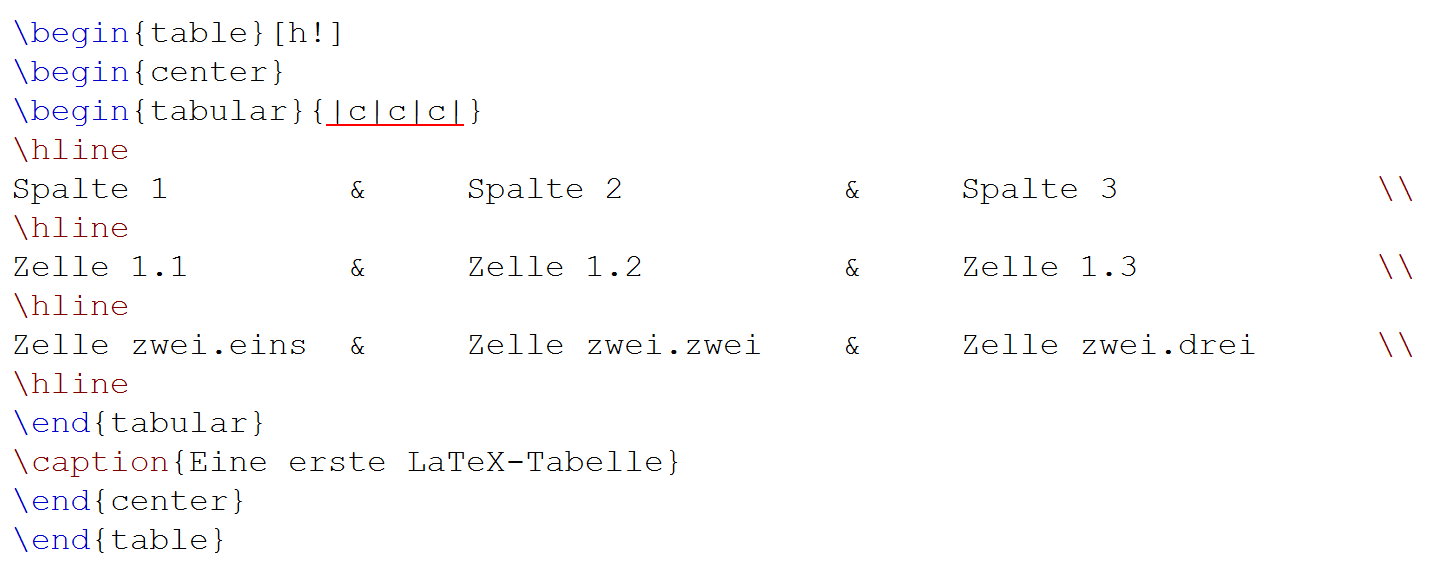
\includegraphics[width=0.75\textwidth]{./Bilder/Tabelle_1.png}}  
      \caption{Eine erste LaTeX-Tabelle}
\end{figure} 

Die Spalten richten sich nach deren Inhalt aus und sind zentriert (c) ausgerichtet, unabhängig davon, wie die einzelnen Spalten in der \code{*.tex}-Datei formatiert sind. 

In folgender Tabelle wollen wir die Spaltenbreite und die Spaltenausrichtung selber kontrollieren. Das Ergebnis sieht wie folgt aus:   


\begin{table}[h!]
\begin{center}
\begin{tabular}{p{4.5cm}|C{3.5cm}|R{4.5cm}}
Spalte 1              &   Spalte 2            &   Spalte 3                \\ 
\hline
Linksbündig           &   Zentriert           &   Rechtsbündig            \\  
\hline
linksbündige Spalte   &   zentrierte Spalte   &   rechtsbündige Spalte    \\ 
\end{tabular}
\caption{Eine zweite LaTeX-Tabelle}
\end{center}
\end{table}



Der dazu benötigte Code:

\begin{figure}[h!]
    \centering
      \fbox{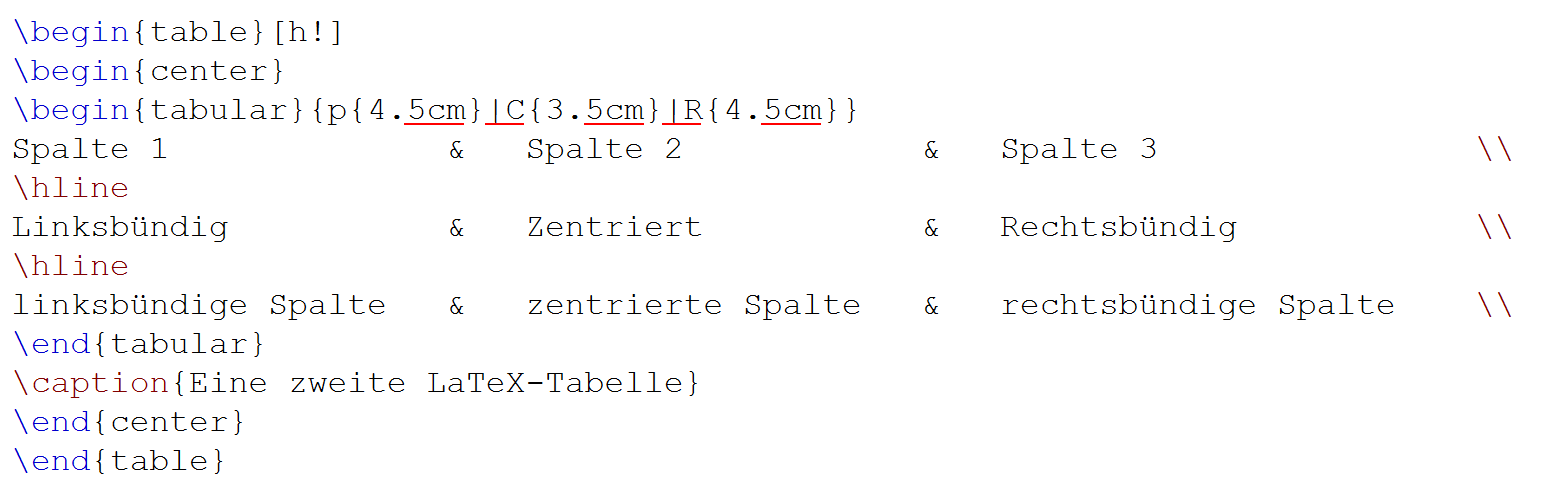
\includegraphics[width=0.75\textwidth]{./Bilder/Tabelle_2.png}}  
      \caption{Eine zweite LaTeX-Tabelle}
\end{figure} 

Der hier gezeigte Code funktioniert nur, wenn in der Präambel die hier verwendeten Befehle eigenhändig definiert werden.

\begin{figure}[h!]
    \centering
      \fbox{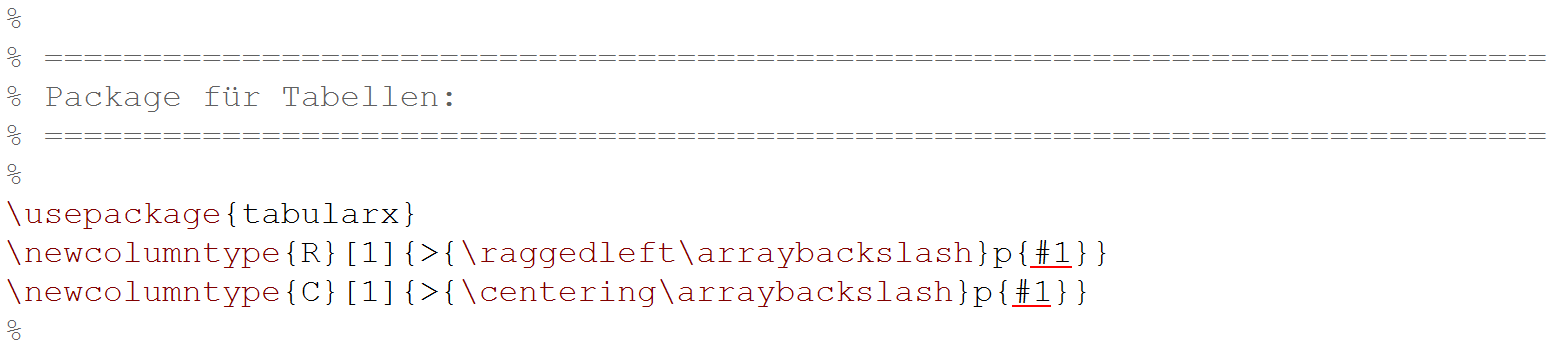
\includegraphics[width=0.75\textwidth]{./Bilder/Tabelle_Praeambel.png}}  
      \caption{LaTeX-Tabellen Präambel}
\end{figure} 

Hier noch ein Beispiel mit verschiedenen Schriftarten in den Zellen und anderen Linien für die Separierung der Zeilen.


\begin{table}[h!]
\begin{center}
\begin{tabular}{p{2cm} C{2cm} R{2cm}}
\toprule
\textbf{Wer}    &    Wo     &    \textit{Was}     \\ 
\midrule
\textbf{ich}    &    da     &    \textit{dies}    \\  
\textbf{du}     &    hier   &    \text{das}       \\ 
\bottomrule
\end{tabular}
\caption{Eine dritte LaTeX-Tabelle}
\end{center}
\end{table}



\newpage
Der hierfür benötigte Code:

\begin{figure}[h!]
    \centering
      \fbox{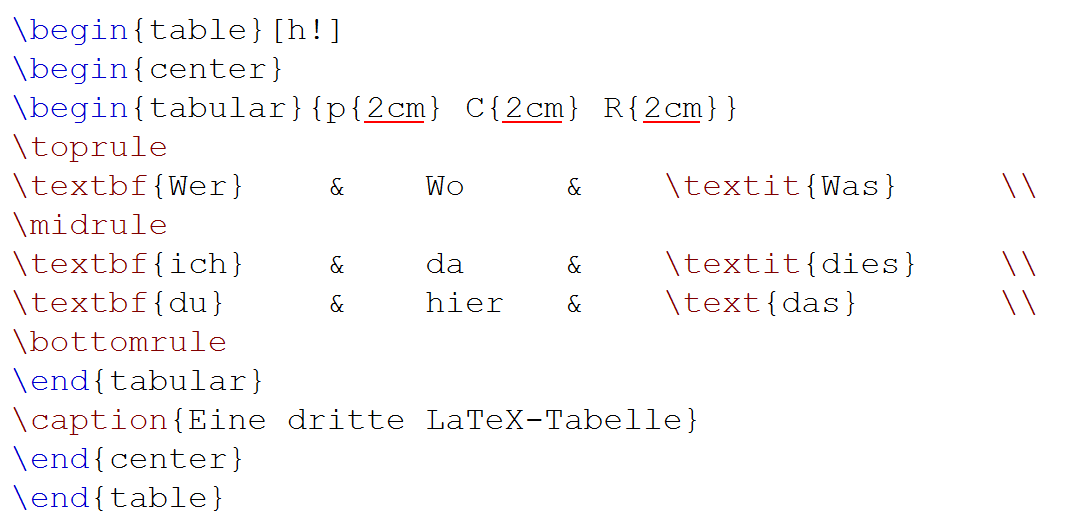
\includegraphics[width=0.75\textwidth]{./Bilder/Tabelle_3.png}}  
      \caption{Eine dritte LaTeX-Tabelle}
\end{figure} 
